\documentclass[a4paper,titlepage]{article}

\usepackage{caption}
\usepackage{subcaption}
\usepackage{graphicx}
\usepackage[utf8]{inputenc}
\usepackage[italian]{babel}
\usepackage[T1]{fontenc}
\graphicspath{ {images/} }

\title{Relazione del Progetto Laboratorio di ASD\\[0.5em]
\large Prima Parte}
\date{Giugno 2021}
\author{
M. Giunta\thanks{Marco Giunta 147852 giunta.marco@spes.uniud.it} \and
S. Anzolin\thanks{Samuele Anzolin 142766  anzolin.samuele@spes.uniud.it} \and
F. Casani\thanks{Federico Casani 141212  casani.federico@spes.uniud.it} \and
G. De Nardi \thanks{Gianluca Giuseppe Maria De Nardi 142733 142733@spes.uniud.it}
}
% Disable indentation
\setlength{\parindent}{0pt}

\begin{document}
% Generate title page
\maketitle

% Generate TOC
\pagenumbering{arabic}
\tableofcontents
\newpage

\section{Introduzione}
In questo progetto abbiamo implementato e analizzato due algoritmi per il calcolo del periodo frazionario minimo di una stringa.
I due algoritmi implementati sono:
\begin{itemize}
  \item \textit{PeriodNaive}
  \item \textit{PeriodSmart}
\end{itemize}
Il linguaggio di programmazione che abbiamo utilizzato per questo progetto è C, in quanto è un linguaggio veloce ed efficiente e qualitativamente migliore per un’analisi temporale.

\section{Ipotesi}
Essendo \textit{periodNaive} un algoritmo con complessità asintotica nel caso peggiore pari a \(O(n^2)\) mentre il secondo raggiunge una complessità lineare, possiamo dedurre
che \textit{periodSmart} sarà notevolmente migliore nel caso peggiore.
\newpage

\section{Implementazione}

\subsection{periodNaive}

L’implementazione di questo algoritmo come dice il suo nome, è abbastanza intuitiva.

Utilizziamo quindi un ciclo che scandisca l’intera stringa di input e internamente controlliamo la congruenza tra il prefisso e il suffisso precedentemente calcolato aumentando la lunghezza del bordo minimo man mano che il ciclo e il controllo avanzano.

\subsection{periodSmart}

Questo algoritmo invece, sfrutta il concetto di bordo, cioè una qualsiasi stringa che sia, prefisso e suffisso proprio della stringa principale.
Come osservato quindi \textbf{p} è un periodo frazionario di \textbf{s} solo se \(p = |s| - r\) dove \textbf{r} è la lunghezza di un bordo di \textbf{s}, quindi il problema si riduce al solo calcolo del bordo massimo della stringa \textbf{s}.

Andiamo quindi ad analizzare l’implementazione vera e propria dell’algoritmo in questione, avremo quindi un algoritmo \textit{searchLongestBorder} che calcola il bordo di lunghezza massima e un algoritmo \textit{periodSmart} che sottrae semplicemente la lunghezza del bordo massimo alla lunghezza della stringa di input per ottenere il periodo frazionario minimo che stiamo cercando.

\subsection{Algoritmo per il calcolo dei tempi medi}

L’algoritmo per il calcolo dei tempi medi richiede di generare delle stringhe di lunghezza compresa tra 1000 e 500000 caratteri e appartenente ad un alfabeto ternario.
Abbiamo utilizzato due metodi per la generazione delle stringhe:
\begin{itemize}
  \item Nel primo caso i caratteri della stringa vengono generati in modo casuale
  \item Il secondo caso, invece, genera una porzione della stringa e la ripete per tutta la lunghezza totale
\end{itemize}
Abbiamo utilizzato la funzione \textit{clock\_gettime} per ottenere il clock necessario al calcolo.
La funzione richiede due parametri, il primo indica il tipo di clock, mentre il secondo contiene il puntatore di una \textit{struct} contenente il tempo all’istante della chiamata a funzione.
Il tipo di clock utilizzato è CLOCK\_MONOTONIC che appunto come suggerisce il nome, è di tipo monotonico.
Dovendo avere un errore relativo massimo di 0,001, dovremo reiterare fino a quando l’equazione:

\[diff(Start,end) < Resolution * (\frac{1}{0,001}+1)\]

\noindent non è più soddisfatta ed inseriremo i dati ottenuti all’interno dei grafici.
\newpage

\section{Analisi dei dati ottenuti}

\subsection{Grafico dei tempi di periodNaive}

\begin{figure}[h]
  \centering
  \begin{subfigure}{\textwidth}
     \captionsetup{justification=centering}
     \caption{Periodo non distribuito}
     \makebox[\textwidth][c]{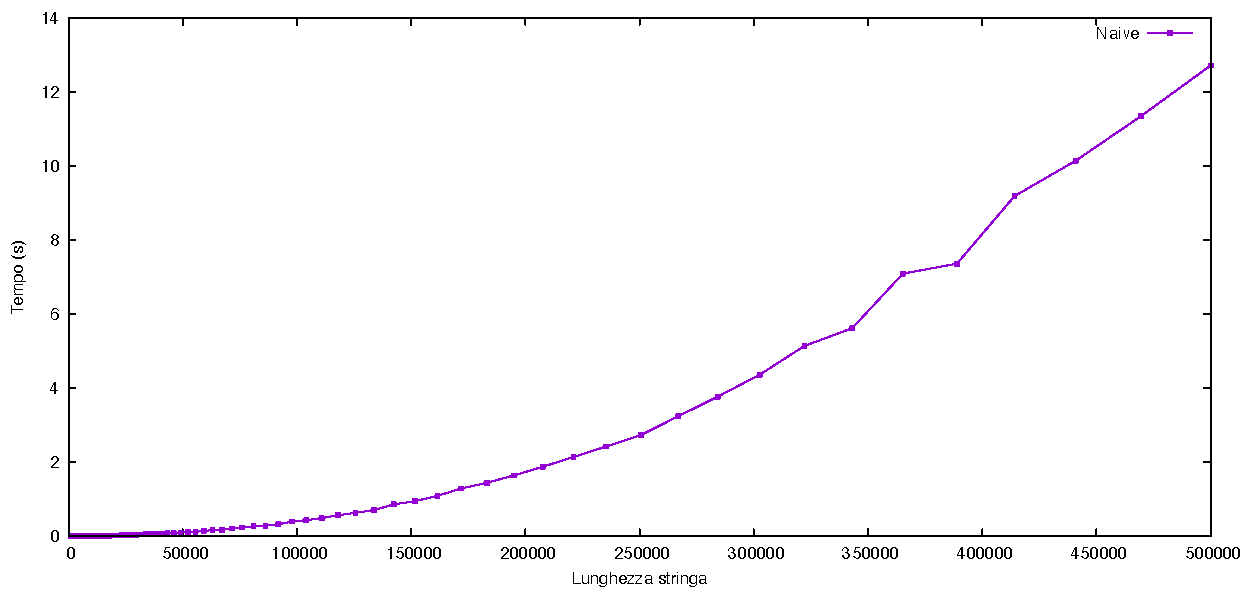
\includegraphics[width=1.24\textwidth]{naive}}%
     \label{fig:naive}
  \end{subfigure}%
  \vspace{2pt}
  \begin{subfigure}{\textwidth}
     \captionsetup{justification=centering}
     \caption{Periodo distribuito}
     \makebox[\textwidth][c]{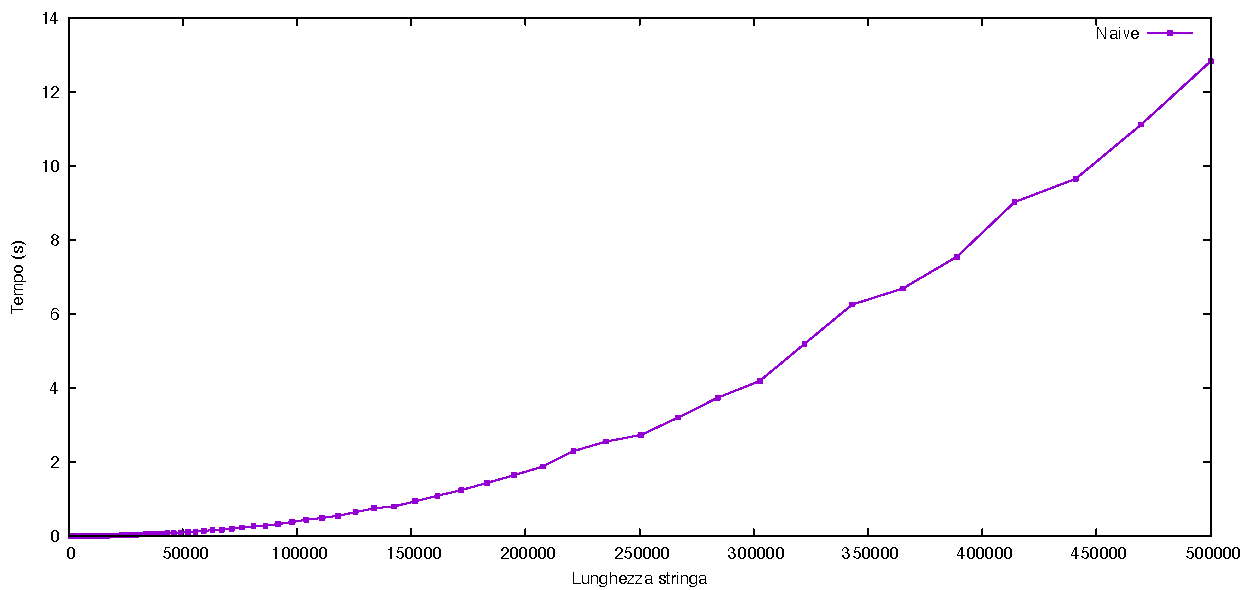
\includegraphics[width=1.24\textwidth]{naive_dist}}%
     \label{fig:naive_dist}
  \end{subfigure}
  \caption{Tempi di calcolo del periodo con algoritmo naive}
\end{figure}
Come possiamo osservare dai due grafici (Figura~\ref{fig:naive} e Figura~\ref{fig:naive_dist} ), il tempo di esecuzione dell’algoritmo \textit{periodNaive} impiega più di dieci secondi per stringhe con più di 450000 caratteri.
\newpage

\subsection{Grafico dei tempi di periodSmart}

\begin{figure}[h]
  \centering
  \begin{subfigure}{\textwidth}
    \captionsetup{justification=centering}
    \caption{Periodo non distribuito}
     \makebox[\textwidth][c]{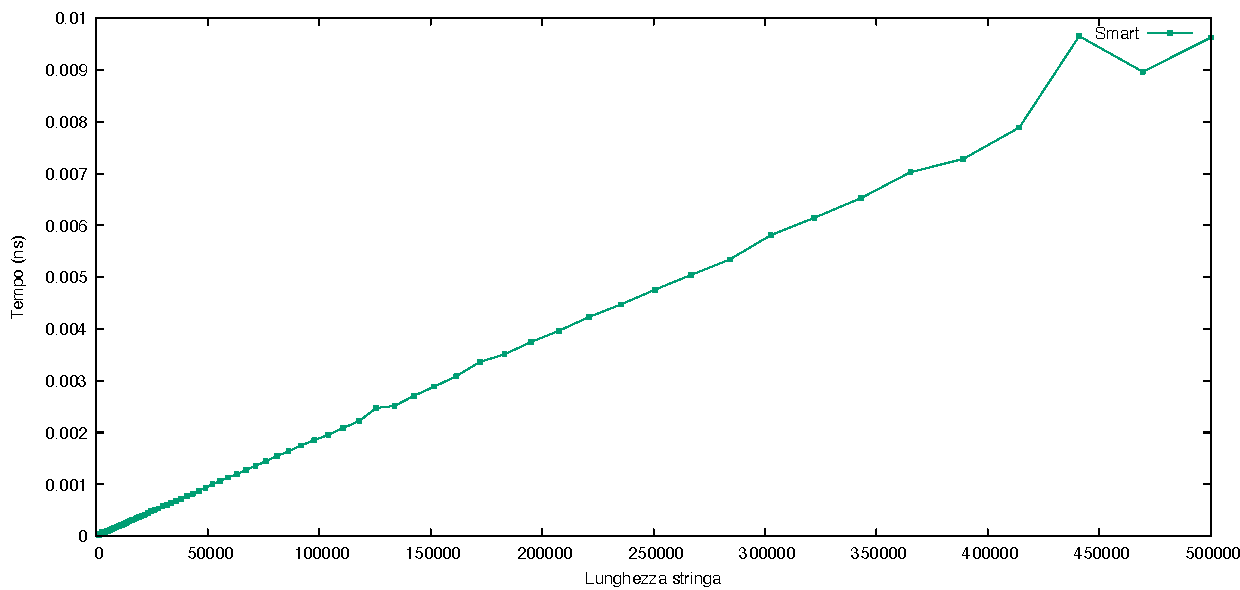
\includegraphics[width=1.24\textwidth]{smart}}%
     \label{fig:smart}
  \end{subfigure}%
   \vspace{2pt}
  \begin{subfigure}{\textwidth}
    \captionsetup{justification=centering}
     \caption{Periodo distribuito}
     \makebox[\textwidth][c]{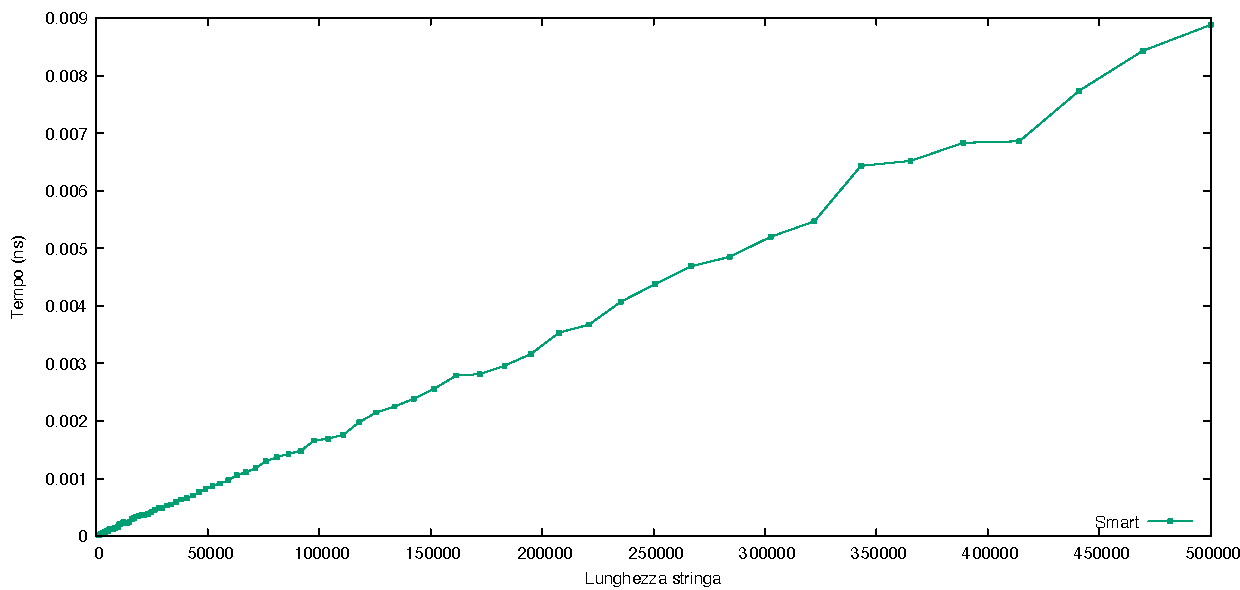
\includegraphics[width=1.24\textwidth]{smart_dist}}%
     \label{fig:smart_dist}
  \end{subfigure}
  \caption{Tempi di calcolo del periodo con algoritmo smart}
\end{figure}

\textit{periodSmart}, invece, impiega un tempo nettamente inferiore per stringhe con una grande quantità di caratteri, parliamo di nanosecondi.
\newpage

\subsection{Analisi logaritmica dei due algoritmi}

\begin{figure}[h]
  \centering
  \begin{subfigure}{\textwidth}
    \captionsetup{justification=centering}
     \caption{Periodo non distribuito}
     \makebox[\textwidth][c]{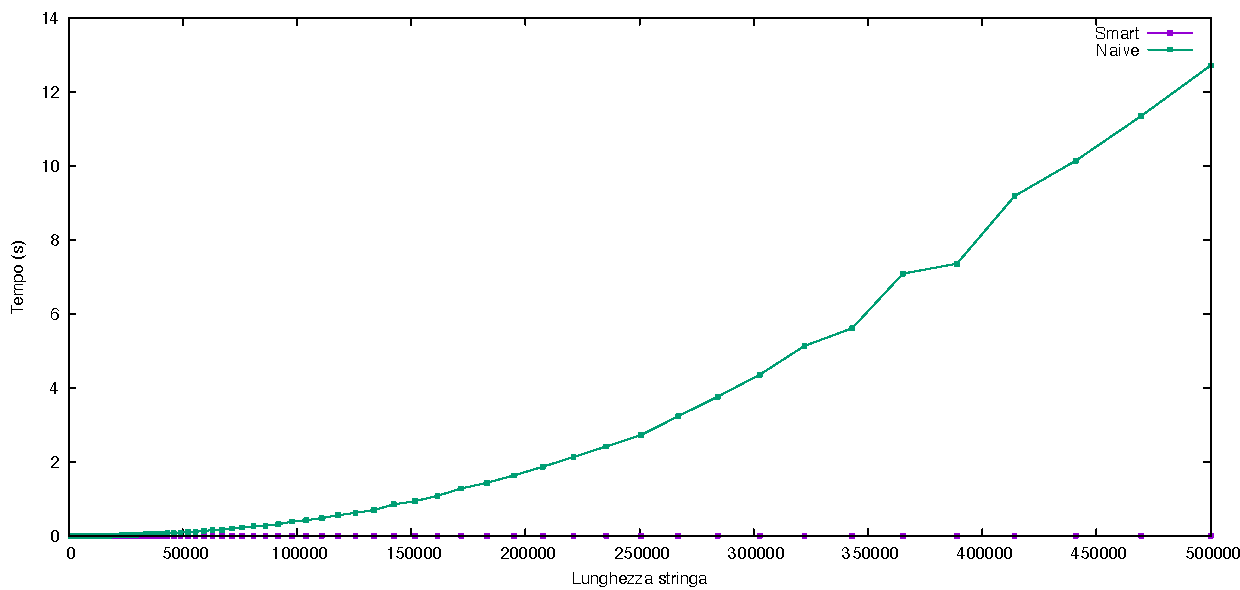
\includegraphics[width=1.2\textwidth]{smart_naive}}%
     \label{fig:smart_naive}
  \end{subfigure}%
  \vspace{2pt}
  \begin{subfigure}{\textwidth}
    \captionsetup{justification=centering}
     \caption{Periodo distribuito}
     \makebox[\textwidth][c]{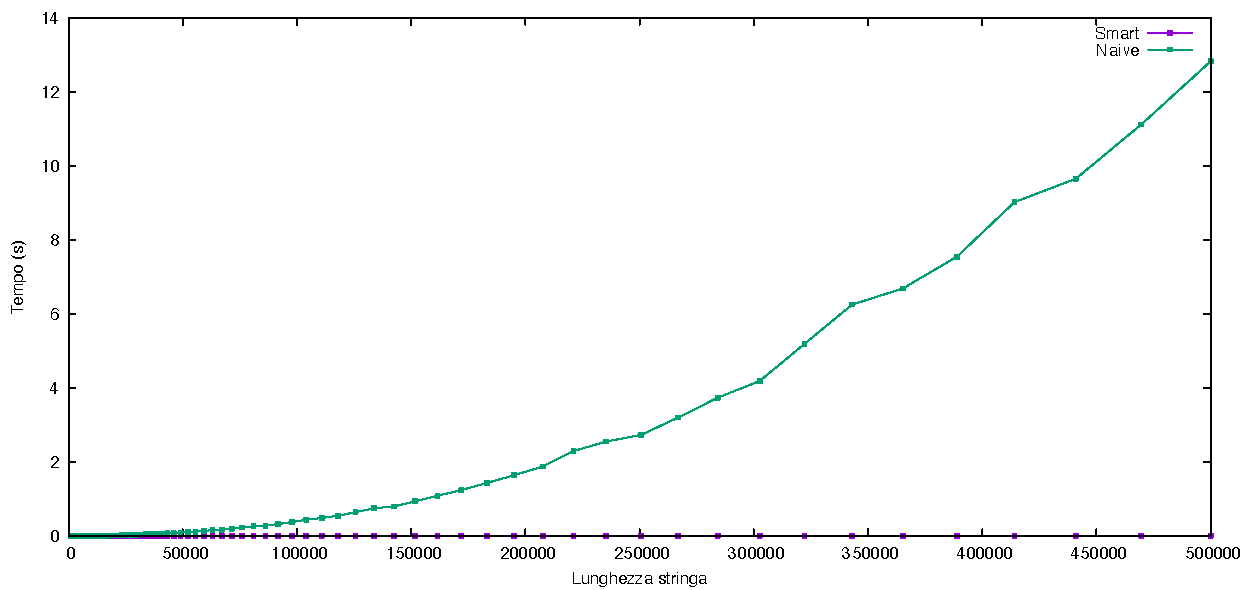
\includegraphics[width=1.2\textwidth]{smart_naive_dist}}%
     \label{fig:smart_naive_dist}
  \end{subfigure}
  \caption{Confronto tempi di calcolo del periodo tra algoritmo smart e algoritmo naive}
\end{figure}

Non potendo analizzare i due algoritmi, visto che sono due scale temporali completamente differenti, dobbiamo quindi analizzarli in una scala logaritmica.
\newpage

\begin{figure}[h]
  \centering
  \begin{subfigure}{\textwidth}
    \captionsetup{justification=centering}
     \caption{Periodo non distribuito}
     \makebox[\textwidth][c]{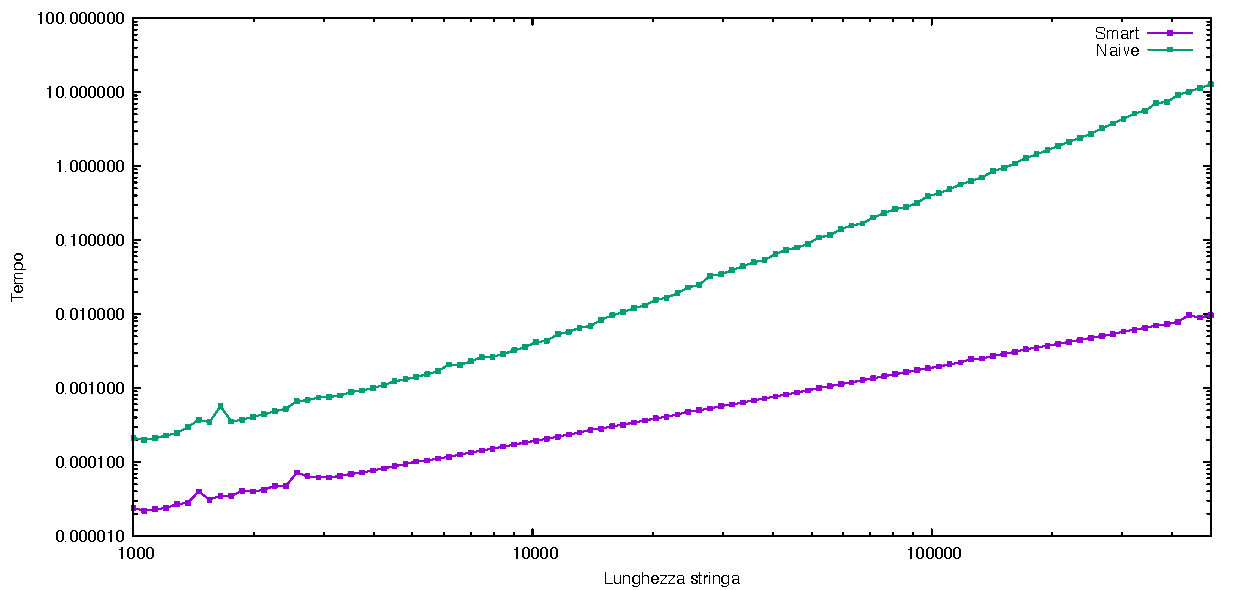
\includegraphics[width=1.2\textwidth]{smart_naive_log}}%
     \label{fig:smart_naive_log}
  \end{subfigure}%
  \vspace{2pt}
  \begin{subfigure}{\textwidth}
    \captionsetup{justification=centering}
    \caption{Periodo distribuito}
     \makebox[\textwidth][c]{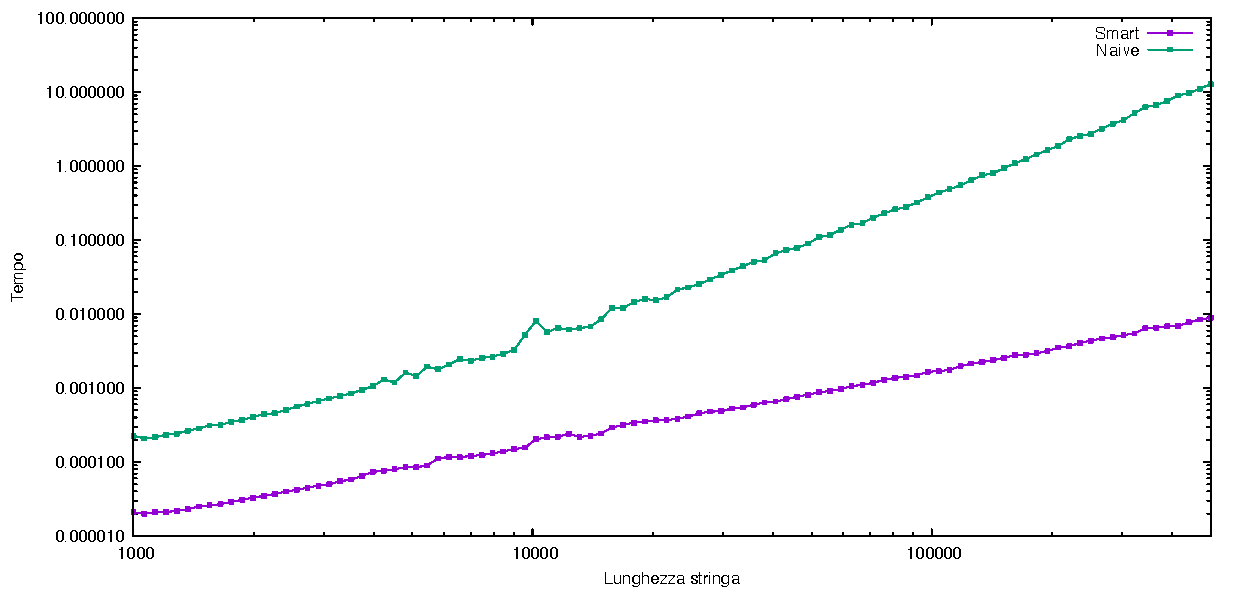
\includegraphics[width=1.2\textwidth]{smart_naive_log_dist}}%
     \label{fig:smart_naive_log_dist}
  \end{subfigure}
  \caption{Confronto tempi di calcolo del periodo tra algoritmo smart e algoritmo naive}
\end{figure}

Non vi sono grossissime differenze con stringhe molto piccole, tuttavia più la stringa di input cresce, più la differenza di tempo tra i due algoritmi aumenta.
\newpage

\subsection{Analisi comparativa tra i due algoritmi}

\begin{figure}[h]
  \centering
  \begin{subfigure}{\textwidth}
    \captionsetup{justification=centering}
     \caption{Periodo non distribuito}
     \makebox[\textwidth][c]{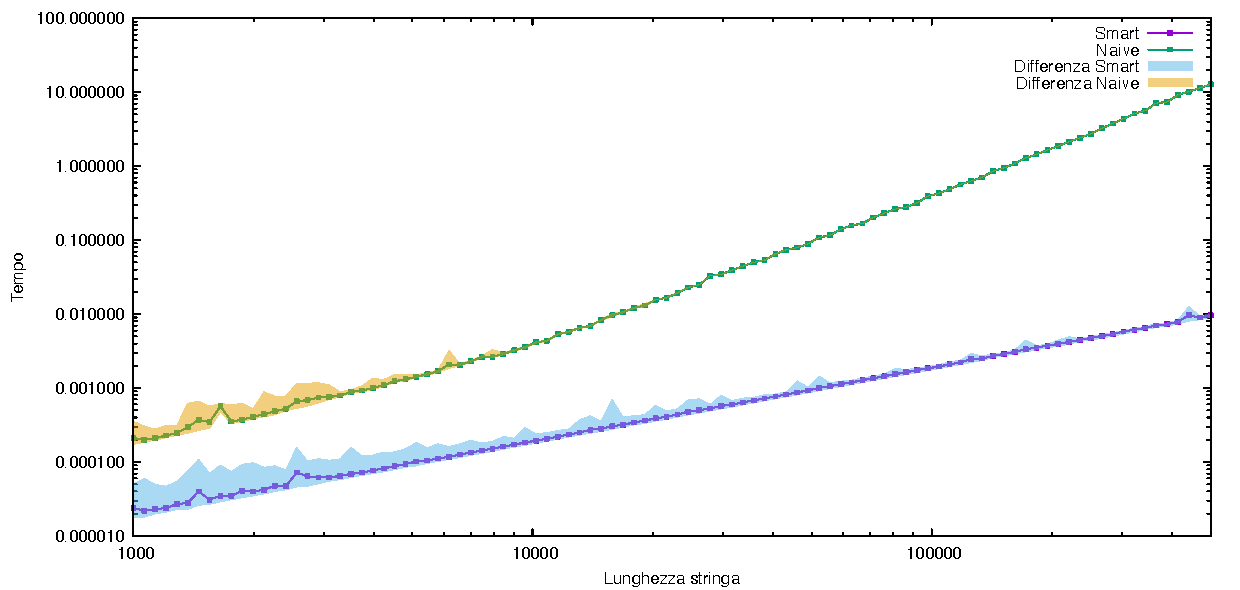
\includegraphics[width=1.2\textwidth]{smart_naive_log_fill}}%
     \label{fig:smart_naive_log_fill}
  \end{subfigure}%
  \vspace{2pt}
  \begin{subfigure}{\textwidth}
    \captionsetup{justification=centering}
    \caption{Periodo distribuito}
     \makebox[\textwidth][c]{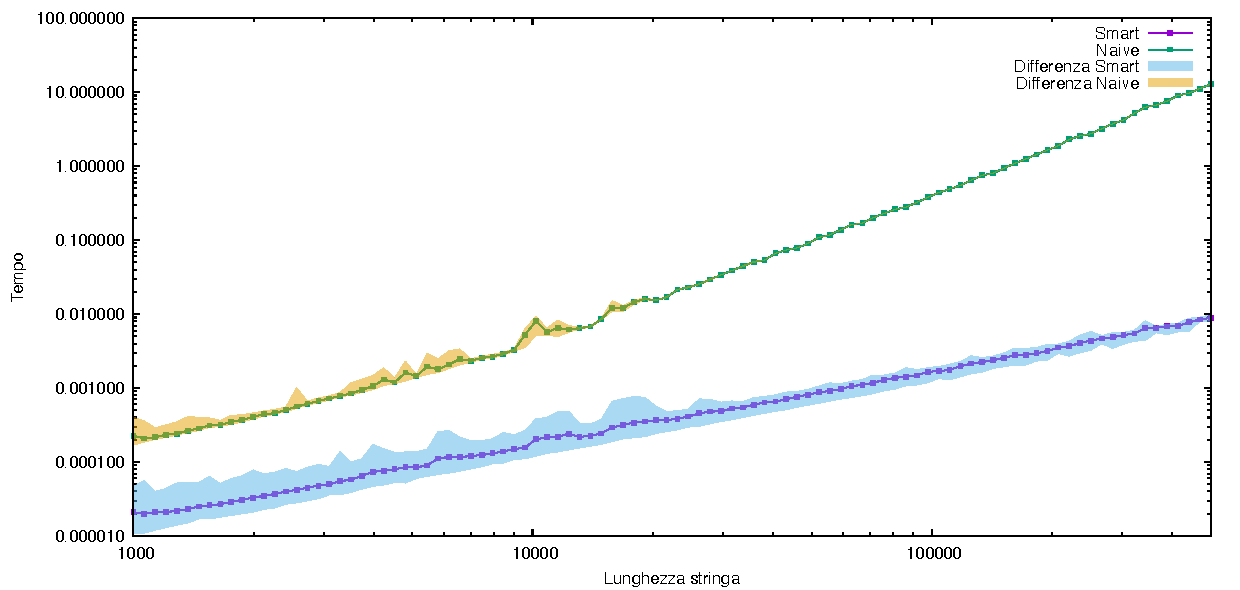
\includegraphics[width=1.2\textwidth]{smart_naive_log_dist_fill}}%
     \label{fig:smart_naive_log_dist_fill}
  \end{subfigure}
  \caption{Confronto tempi di calcolo del periodo tra algoritmo smart e algoritmo naive}
\end{figure}

Dai grafici qui sopra possiamo notare come, l’errore relativo massimo, influenzi il numero di rilevazioni che andiamo a fare.
Infatti, nel caso di \textit{periodNaive} il numero di rilevazioni raccolte scende a uno dopo una certa soglia, mentre \textit{periodSmart} continua a effettuare più di una rilevazione anche quando l’input raggiunge dimensioni considerevoli.
Questo ad indicare che i tempi di \textit{periodSmart} sono molto ridotti.
\newpage

\section{Conclusioni}

Come osservato dai grafici, abbiamo sicuramente costatato che tra i due algoritmi c’è una notevole differenza in termini di tempo.
L’argoritmo \textit{periodSmart} impiega molto meno tempo dell'algoritmo \textit{periodNaive}  ed è quindi più consigliato il suo utilizzo.
\end{document}
